\cleardoublepage
\chapter{Domänenmodellierung -- Klassen und Objekte}
\label{sec:Kap-4}

Es gibt sehr viele unterschiedliche Möglichkeiten, Modelle im Softwareengineering einzusetzen. Wichtig für ein Softwareentwicklungsprojekt ist, das Modellieren nicht zum Selbstzweck werden zu lassen, sondern Modelle immer als Schritte auf dem Weg zum zu erstellenden Softwareprodukt zu sehen und somit sowohl quantitativ als auch qualitativ \textbf{zielgerichtet} zu modellieren. Das betrifft auch die Realweltmodellierung, mit der wir in diesem Kapitel beginnen. Man erstellt Modelle der Realwelt nicht, um ein hübsches Bild von den Zuständen der Wirklichkeit zu erhalten, sondern weil man ein Softwareprodukt entwickeln möchte, das \textbf{in} dieser Wirklichkeit \textbf{oder mit} dieser Wirklichkeit arbeitet.

Das Modellieren
\marginline{Modellieren ist subjektiv}
von Sachverhalten – seien es Realweltzusammenhänge oder Entwurfsentscheidungen für die Implementierung – ist stets eine subjektive Handlung. Von ganz trivialen Beispielen einmal abgesehen, können identische Sachverhalte von verschiedenen Modellierern unterschiedlich modelliert werden. Es gibt durchaus Heuristiken, an denen man sich als Modellierer orientieren kann („üblicherweise“), aber keine Formel für das ideale Diagramm. Die UML unterstützt durch die mittlerweile recht ausgereifte inhaltliche Abgrenzung ihrer unterschiedlichen Modellierungs\-elemente aber eine gewisse Standardisierung.


%--- Kapitel 4.1 - 4.3
\clearpage
\section{Realwelt-Objekte modellieren}
\label{sec:Kap-4.1}

Im objektorientierten Softwareengineering versucht man das (zukünftige) Softwareprodukt so zu gestalten, dass es sich an den Objekten und Strukturen der Domäne orientiert. Die UML bietet mit dem sogenannten \textit{Objektdiagramm}
\marginline{Objekt\-diagramm} 
die Möglichkeit, (Abstraktionen der) Objekte der Realwelt, ihre Eigenschaften und ihre Beziehungen zueinander in einer von UML vorgegebenen Syntax zu modellieren. Objektdiagramme können unterschiedlich umfangreich sein, auch eine Menge von Objekten ohne Verbindungen zueinander (wie in Abbildung~\ref{fig:objektdiagramm_unverbundene_objekte}) und selbst ein einziges aufgezeichnetes Objekt (wie in Abbildung~\ref{fig:objekt_in_uml-darstellung}) stellen Objektdiagramme dar. In der praktischen Anwendung im Softwareengineering beinhalten Objektdiagramme in der Regel aber mehrere verbundene Objekte. 

Zu modellierende Realwelt-Objekte \marginline{Objekt}
können Dinge sein, die man sehen oder anfassen kann, wie zum Beispiel eine Katze, ein Tisch, eine Person oder ein Stern, aber auch immaterielle Dinge, wie zum Beispiel ein Konto, eine Reise oder eine Vorlesung. In der UML-Notation werden Objekte als rechteckige Kästen dargestellt, die (mindestens, s.u.) einen Objektnamen enthalten.

\vspace{2mm} %%% für Druck

\begin{figure}[h!]
	\centering
	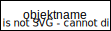
\includegraphics{Bilder/Kapitel-4/objekt_in_uml-darstellung.pdf}
	\caption{Ein Objekt in UML-Darstellung}
	\label{fig:objekt_in_uml-darstellung}
\end{figure}

Nach UML-Konvention wird der Objektname unterstrichen dargestellt. Üblich – obwohl die UML diesbezüglich keine Vorgaben macht – ist außerdem, dass Objektnamen mit einem Kleinbuchstaben beginnen und zentriert dargestellt werden. Innerhalb eines Diagramms müssen die Objektnamen eindeutig gewählt werden. Sollten innerhalb eines Diagramms trotzdem zwei Kästchen denselben Namen enthalten – die UML verbietet dies nicht –, so ist mit beiden Kästchen dasselbe Objekt gemeint. Die doppelte Darstellung eines Objekts wird vor allem in handschriftlich erstellten oder sehr umfangreichen Objektdiagrammen aus Lesbarkeitsgründen verwendet.

\vspace{2mm} %%% für Druck

\begin{figure}[h!]
	\centering
	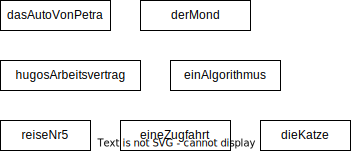
\includegraphics{Bilder/Kapitel-4/objektdiagramm_unverbundene_objekte.pdf}
	\caption{Ein Objektdiagramm mit sieben unverbundenen Objekten}
	\label{fig:objektdiagramm_unverbundene_objekte}
\end{figure}

Abbildung~\ref{fig:objektdiagramm_unverbundene_objekte} zeigt weitere Objekte in UML-Darstellung. Bei manchen wird aus dem Namen (relativ) deutlich, welches konkrete Realwelt-Objekt gemeint ist. So ist \linebreak \sttpUMLText{dasAutoVonPetra}, sofern man Petra kennt und sie nicht mehr als ein Auto besitzt, einem konkreten Realwelt-Auto zuordenbar. Für \sttpUMLText{reiseNr5} bedarf es dagegen schon der zusätzlichen Kenntnis des Kontexts (\zb die Auflistung von Reisen in einem Katalog), um eine Realwelt-Reise mit diesem Namen zu verbinden. Für Objekte wie \sttpUMLText{einAlgorithmus} oder \sttpUMLText{eineZugfahrt} und auch \sttpUMLText{dieKatze} lassen sich die gemeinten Realweltentsprechungen nicht bestimmen. 

Zumindest könnte man aber anhand der Namen der Objekte vielleicht auf die \textbf{Art} des Realwelt-Objekts schließen? So sollte es sich bei \sttpUMLText{dieKatze} doch wohl um eine Katze und nicht um einen Hund handeln? Doch vielleicht trägt mein Realwelt-Meerschweinchen – aus welchem Grund auch immer – den Namen \sttpUMLText{dieKatze} und meine Realwelt-Katze heißt stattdessen \sttpUMLText{pünktchen}. Der modellierten Abstraktion des Realwelt-Objekts kann man den Typ des Objekts in der bisher gewählten Darstellungsform also nicht ansehen. 

Um den Typ eines modellierten Realwelt-Objekts anzugeben, wird in der UML-Dar\-stel\-lung des Objekts der Objektname um die Angabe des Namens der \textit{Klasse}
\marginline{Klasse}
ergänzt (Abb.~\ref{fig:darstellung_objekt} rechts). Die Objektdarstellung ohne zusätzlichen Klassennamen (wie in Abb.~\ref{fig:darstellung_objekt} links und den vorherigen Abbildungen) ist nach UML-Regeln zulässig, sollte aus semantischen Gründen aber nur dann verwendet werden, wenn der Zielgruppe des Modells der Typ des Objekts bekannt ist.

\begin{figure}[h!]
	\centering
	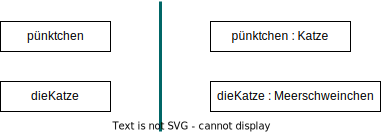
\includegraphics{Bilder/Kapitel-4/darstellung_objekt.pdf}
	\caption[Ein Katzen-Objekt namens \sttpUMLText{pünktchen} und ein Meerschweinchen-Objekt namens \sttpUMLText{dieKatze}]{Ein Objekt namens \sttpUMLText{pünktchen} und ein Objekt namens \sttpUMLText{dieKatze} (links). Ein Katzen-Objekt namens \sttpUMLText{pünktchen} und ein Meerschweinchen-Objekt namens \sttpUMLText{dieKatze} (rechts). Der senkrechte Strich in der Abbildung trennt die linke und die rechte Seite dieser Abbildung. Er ist nicht Bestandteil eines UML-Objektdiagramms.}
	\label{fig:darstellung_objekt}
\end{figure}


\sttpHinweiskasten{1.0}{CamelCase-Schreibweise}{Bezeichner (Namen) in Programmcode dürfen häufig keine Leerzeichen enthalten. Die sogenannte CamelCase-Schreibweise, bei der das erste Wort kleingeschrieben wird und alle folgenden jeweils mit einem Großbuchstaben beginnen, ist eine Möglichkeit, auch ohne Trennzeichen ausdrucksstärkere Bezeichner als \zb \sttpUMLText{auto1} und \sttpUMLText{auto2} zu verwenden. Die CamelCase-Schreibweise findet man auch in Domänenmodellen häufig, obwohl Domänenmodelle eigentlich noch von Implementierungsaspekten abstrahieren sollten und hier die Verwendung von Leerzeichen Realwelt-näher wäre. Die UML selber macht keine Vorgaben oder Einschränkungen bezüglich der Schreibweise der Namen, spezifische UML-Werkzeuge tun dies allerdings teilweise schon.}

Abbildung~\ref{fig:sechs_mal_katze} zeigt weitere Katzen-Objekte. Wichtig ist, dass jeweils ausschließlich die Angabe \sttpUMLText{:Katze} bestimmt, dass es sich um ein Objekt vom Typ Katze handelt. Die beiden unteren Objekte in der Abbildung sind sogenannte \textit{anonyme Objekte}.
\marginline{anonymes Objekt}
Diese Form der Darstellung wird verwendet, wenn man nicht ein konkretes, mit einem Namen versehenes, Katzen-Objekt modellieren möchte, sondern \textbf{irgendein} Objekt vom Typ Katze. Beachten Sie, dass auch ein anonymes Objekt nur genau \textbf{ein} Objekt ist. Es steht nicht stellvertretend für beliebig viele Katzen-Objekte. Im Unterschied zu benannten Objekten handelt es sich bei mehreren anonymen Objekten derselben Klasse im selben Objektdiagramm nach UML-Definition um \textbf{unterschiedliche} Objekte. Die beiden anonymen Katzen-Objekte in Abbildung~\ref{fig:sechs_mal_katze} modellieren daher zwei unterschiedliche Realwelt-Katzen, bei denen es aber für den Modellierungszweck irrelevant ist, um welche konkreten Realwelt-Katzen es sich handelt. Das Objekt mit Namen \sttpUMLText{eineKatze} ist dagegen kein anonymes Objekt, sondern modelliert genau diejenige Realwelt-Katze, die den Namen \sttpUMLText{eineKatze} trägt.

\begin{figure}[h!]
	\centering
	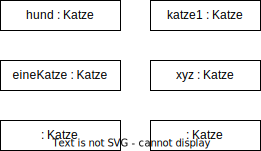
\includegraphics{Bilder/Kapitel-4/sechs_mal_katze.pdf}
	\caption{Vier benannte und zwei anonyme Objekte der Klasse \sttpUMLText{Katze}}
	\label{fig:sechs_mal_katze}
\end{figure}

Das Konzept der Klasse ist ein zentraler Bestandteil der objektorientierten Softwareentwicklung – auch wenn es einige wenige objektorientierte Programmiersprachen gibt (\zb JavaScript), die keine Klassen, sondern ausschließlich Objekte kennen. Sie kennen aus der objektorientierten Programmierung sicher die Definition einer Klasse als Bauplan bzw. Schablone für gleichartige Software-Objekte. Dabei wird die Klasse aus dem Blickwinkel der Programmcodeerstellung betrachtet. Aber was ist eigentlich eine Klasse, wenn wir mit dem Fokus der Realweltmodellierung hinsehen?

Abbildung~\ref{fig:klassenbegriff} greift das Beispiel mit Herrn Müller aus Abschnitt 3.2.1 (S.~\pageref{fig:mueller_lehrer_fussballer}) wieder auf. Aus dem Realwelt-Objekt Herr Müller wird durch entsprechende (unter\-schied\-liche) Abstraktion das modellierte Realwelt-Objekt Lehrer Müller oder das modellierte Realwelt-Objekt Fußballer Müller. Eine Klasse
\marginline{eine Klasse\\ ist die Beschrei\-bung einer Abstrak\-tion}
beschreibt genau diese Abstraktion zwischen dem Realwelt-Objekt und der Modellierung des Realwelt-Objekts. Die Klasse Lehrer definiert, welche Merkmale des Realwelt-Objekts für die Modellierung als Lehrer Müller relevant sind. Die Klasse Fußballer beschreibt die\-jenigen Merkmale des Realwelt-Objekts, die für die Modellierung als Fußballer Müller relevant sind.

\begin{figure}[h!]
	\centering
	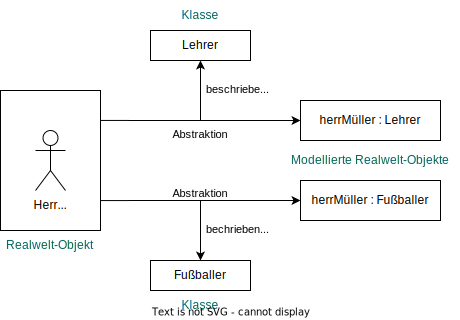
\includegraphics{Bilder/Kapitel-4/klassenbegriff_realweltmodellierung.pdf}
	\caption{Der Klassenbegriff aus Sicht der Realweltmodellierung}
	\label{fig:klassenbegriff}
\end{figure}


Zwei Aspekte zum Konzept der Klasse müssen wir an dieser Stelle noch ergänzen. Erstens gilt die in den Klassen Lehrer und Fußballer beschriebene Abstraktion natürlich nicht nur für das konkrete Realwelt-Objekt Herrn Müller, sondern für alle Realwelt-Objekte (Frau Schulze, Herr Özdemir, Frau Kinsombi,~\ldots), die modellierte Realwelt-Lehrer oder Realwelt-Fußballer werden sollen. Und zweitens beschreibt eine Klasse die Abstraktion zwischen Realwelt-Objekt und Modellierung eines solchen Realwelt-Objekts auch dann, wenn man (noch) gar kein modelliertes Objekt hat. So kann zum Beispiel eine Klasse Katze existieren, die definiert, wie man von einer Realwelt-Katze zu einer modellierten Realwelt-Katze kommen würde, ohne dass es ein modelliertes Katzen-Objekt gibt. Eine Klasse ist somit unabhängig von der Existenz der modellierten Objekte – umgekehrt gilt dies jedoch nicht.

\vspace{\baselineskip} %%% für Druck

\begin{figure}[h!]
	\centering
	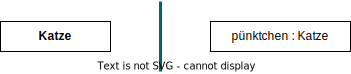
\includegraphics{Bilder/Kapitel-4/darstellung_klasse.pdf}
	\caption[Eine Klasse mit Namen \sttpUMLText{Katze} und ein Objekt dieser Klasse]{Eine Klasse mit Namen \sttpUMLText{Katze} (links) und ein Objekt dieser Klasse mit Namen \sttpUMLText{pünktchen} (rechts)}
	\label{fig:darstellung_klasse}
\end{figure}

\vspace{\baselineskip} %%% für Druck

Die UML-Darstellung einer Klasse ist sehr ähnlich zu der Darstellung eines Objekts. Es handelt sich ebenfalls um ein Rechteck, in dem (mindestens) der Klassenname eingetragen ist. Abbildung~\ref{fig:darstellung_klasse} zeigt links eine Klasse \sttpUMLText{Katze} und rechts ein modelliertes Katzen-Objekt namens \sttpUMLText{pünktchen}. Im Unterschied zu Objekten wird bei der Darstellung einer Klasse der Name nicht unterstrichen. Zudem ist es üblich, den Klassennamen mit einem Großbuchstaben zu beginnen und ihn zentriert und fett gedruckt zu setzen. Der Klassenname ist üblicherweise ein Substantiv im Singular und nicht im Plural. Wie auch bei den benannten Objekten gilt für Klassen in einem Diagramm, dass es sich bei der mehrfachen Darstellung einer Klasse per Defi\-ni\-tion um dieselbe Klasse handelt. Die mehrfache Darstellung von Klassen in einem Diagramm sollte man nur sehr dosiert anwenden, da die existierenden Beziehungen zwischen Klassen (s. Kap. \ref{sec:Kap-4.3}) mit jeder Dopplung einer Klasse im Diagramm weniger gut zu überblicken sind.

Wenn man Softwareprodukte, wie zum Beispiel die erwähnte Schulverwaltungssoftware entwickeln möchte, sind die konkreten Objekte der Realwelt wie Herr Müller meistens weniger interessant. Entscheidender ist, dass die Software später mit beliebigen Objekten eines bestimmten Typs (\zb Lehrer-Objekt) umgehen kann. Die Informationen zu den Merkmalen von Objekttypen finden sich in der objektorientierten Softwareentwicklung aber in den Klassen und nicht in den Objekten. Daher interessieren für die Softwareentwicklung vor allem die Klassen.

Für die Modellierung von Klassen stellt die UML ein eigenes Diagramm, das \textit{Klassen\-diagramm},
\marginline{Einsatzgebiete von Klassen- und Objekt\-diagrammen}
zur Verfügung.  Es gehört wie das Objektdiagramm zu den Struktur\-diagrammen der UML und stellt Klassen und ihre Beziehungen zueinander dar. Das Klassendiagramm ist für das Softwareengineering eine der wichtigsten Diagramm\-arten der UML, da es in fast allen Prozessen des Softwareengineering eingesetzt werden kann. Objektdiagramme dagegen werden in der Praxis seltener eingesetzt. Man kann sie verwenden, um bestimmte Situationen zur Laufzeit des Software\-produkts zu veranschaulichen: Welche Software-Objekte existieren zu einem bestimmten Zeitpunkt und wie stehen sie miteinander in Verbindung. Für die Lehre eignen sich Objekt\-diagramme zudem ganz gut, da sie für Anfänger im Bereich der Objektorientierung die Kluft zwischen den Objekten der Realwelt und den Klassen der objektorientierten Programmierung überbrücken helfen.

\clearpage
\section{Merkmale modellieren}
\label{sec:Kap-4.2}

Merkmale von Realwelt-Objekten, zum Beispiel die Fellfarbe bei Katzen, definiert man in der objektorientierten Softwareentwicklung in den Klassen. Dafür verfügen die Klassen über sogenannte \textit{Attribute}.
\marginline{Attribute}

\vspace{2mm} %%% für Druck

\begin{figure}[h!]
	\centering
	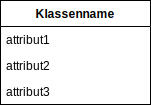
\includegraphics{Bilder/Kapitel-4/darstellung_klasse_mit_drei_attributen.pdf}
	\caption[Die UML-Darstellung einer Klasse]{Die UML-Darstellung einer Klasse mit Angabe des Namens der \mbox{Klasse} und drei Attributen}
	\label{fig:darstellung_klasse_mit_drei_attributen}
\end{figure}

In der UML-Darstellung wird das Rechteck der Klasse durch eine Linie horizontal unterteilt. Oberhalb der Linie steht der schon bekannte Name der Klasse, unterhalb der Linie werden die Attribute, untereinander und linksbündig gesetzt, aufgeführt. Jedes (spätere) Objekt, das nach den Vorgaben der Klasse modelliert wird – man sagt verkürzend: „Jedes Objekt der Klasse“ – verfügt über genau die Attribute, die die Klasse definiert. Die Werte der Attribute, also die Ausprägung der Merkmale, sind dabei jedoch spezifisch pro Objekt.

Wir wechseln von Katzen zu Autos! Abbildung~\ref{fig:klasse_auto_mit_zwei_attributen} zeigt eine Klasse \sttpUMLText{Auto} mit den zwei Attributen \sttpUMLText{modell} und \sttpUMLText{farbe}.

\begin{figure}[h!]
	\centering
	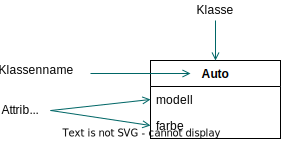
\includegraphics{Bilder/Kapitel-4/klasse_auto_mit_zwei_attributen.pdf}
	\caption{Eine Klasse \sttpUMLText{Auto} mit zwei Attributen}
	\label{fig:klasse_auto_mit_zwei_attributen}
\end{figure}

Abbildung~\ref{fig:drei_mal_klasse_auto_plus_klasse_hugoauto} oben zeigt mit \sttpUMLText{ellensAuto}, \sttpUMLText{heikesAuto} und \sttpUMLText{marvinsAuto} drei Objekte, die die von der Klasse \sttpUMLText{Auto} definierten Merkmale (Vorhandensein der Eigenschaften Modell und Farbe) erfüllen und damit Objekte der Klasse \sttpUMLText{Auto} sind. Die von der Klasse vorgegebenen Attribute sind bei den Objekten mit konkreten Werten belegt: Für das Attribut \sttpUMLText{modell} finden wir hier die Werte Toyota Yaris und VW Golf, für das Attribut \sttpUMLText{farbe} die Werte stahlblau, weiß und rot. Wie hier bei dem \sttpUMLText{modell}-Attribut von \sttpUMLText{ellensAuto} und \sttpUMLText{heikesAuto} können die Werte -- man sagt auch synonym: Wertebelegungen
\marginline{Werte\-belegungen}
-- von Attributen bei unterschiedlichen Objekten auch übereinstimmen. Wenn zwei Objekte derselben Klasse in \textbf{allen} \mbox{Wertebelegungen} der Attribute übereinstimmen, also zum Beispiel Heikes Toyota Yaris auch stahlblau wäre wie der von Ellen, nennt man dies in der Objektorientierung zustandsgleiche Objekte.

\begin{figure}[h!]
	\centering
	\includegraphics{Bilder/Kapitel-4/klasse_auto.pdf}
	\caption[Drei Objekte der Klasse \sttpUMLText{Auto}]{Drei Objekte der Klasse \sttpUMLText{Auto} (oben) und ein Objekt mit Namen \sttpUMLText{hugosAuto}, das kein Objekt der Klasse Auto aus Abbildung~\ref{fig:klasse_auto_mit_zwei_attributen} ist (unten)}
	\label{fig:drei_mal_klasse_auto_plus_klasse_hugoauto}
\end{figure}

Abbildung~\ref{fig:drei_mal_klasse_auto_plus_klasse_hugoauto} unten
\marginline{der Unterschied zwischen Realwelt-Objekten und modellierten Objekten}
zeigt ein Objekt mit Namen \sttpUMLText{hugosAuto}, das im Gegensatz zu den drei anderen Objekten kein Objekt der in Abbildung~\ref{fig:klasse_auto_mit_zwei_attributen} modellierten Klasse \sttpUMLText{Auto} ist, da es über ein Attribut \sttpUMLText{baujahr} verfügt, das die in Abbildung~\ref{fig:klasse_auto_mit_zwei_attributen} dargestellte Auto-Klasse nicht kennt. An dieser Stelle müssen Sie sich noch einmal den Unterschied zwischen Realwelt-Objekten und den für Softwareengineering-Zwecke modellierten Objekten vergegenwärtigen: Das Realwelt-Auto von Hugo ist sicher genau wie die Autos von Ellen, Heike und Marvin ein Auto. Und die Realwelt-Autos der drei letzteren Personen haben auch genau wie Hugos Auto ein Baujahr. Die in Abbildung~\ref{fig:klasse_auto_mit_zwei_attributen} für einen (hier unbekannten) Zweck im Rahmen des Softwareengineering modellierte Klasse Auto abstrahiert von allen Eigenschaften von Realwelt-Autos, die für den Modellierungszweck nicht relevant sind. Und in diesem Beispiel betrifft das eben auch das Merkmal Baujahr. \textbf{Modellierte} Objekte vom Typ Auto besitzen hier daher kein Attribut \sttpUMLText{baujahr}, auch wenn für ihre Realweltentsprechungen ein Baujahr existiert.

An dem Auto-Baujahr-Beispiel zeigt sich ein weiterer praktischer Verwendungszweck von Objektdiagrammen. In  Diskussionen über die relevanten Strukturen der Domäne zwischen Softwareentwicklungsteam und Kunden kann es für die Kunden schwierig sein, die ihnen bekannte Ebene der Realwelt-Objekte mit der Ebene der deutlich abstrakteren Klassen zusammenzubringen. Hier kann es helfen, statt Klassen zunächst konkrete (Beispiel)Objekte und ihre Eigenschaften zu modellieren und erst anschließend auf dieser Grundlage die benötigten Klassen zu entwerfen.

\clearpage
\section{Beziehungen modellieren}
\label{sec:Kap-4.3}

Um in UML-Objektdiagrammen eine Beziehung zwischen Objekten zu modellieren, verbindet man die Kästen der Objekte mit einer durchgezogenen Linie. Die UML-Termi\-no\-logie für eine Beziehung von Objekten ist \textit{Verbindung} (engl. link). \marginline{Objekt\-verbindungen} Abbildung~\ref{fig:objektdiagramm} zeigt ein Objektdiagramm, das zwei Lehrer-Objekte, drei Fach-Objekte und drei Schüler-Objekte enthält. Zwischen einigen der Objekte bestehen Verbindungen. So hat zum Beispiel das Lehrer-Objekt mit Namen \sttpUMLText{weber} oben links eine Verbindung zum Fach-Objekt \sttpUMLText{sport} und eine weitere zum Fach-Objekt \sttpUMLText{biologie}. Anhand des Namens der Verbindung (\sttpUMLText{unterrichtet}) erkennt man, welche Art von Realweltbeziehung hier abgebildet wird: Der Realwelt-Lehrer Weber unterrichtet die Fächer Sport und Biologie. 

\vspace{\baselineskip} %%% für Druck

\begin{figure}[h!]
	\centering
	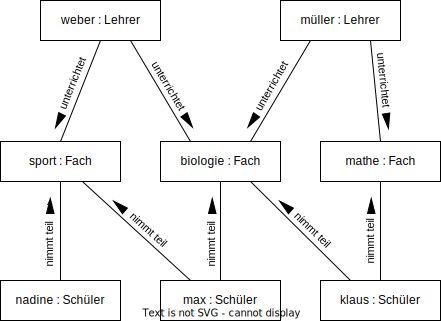
\includegraphics{Bilder/Kapitel-4/objektdiagramm_lehrer_fach_schueler.pdf}
	\caption{Ein Objektdiagramm}
	\label{fig:objektdiagramm}
\end{figure}

\vspace{\baselineskip} %%% für Druck

Das kleine schwarze Dreieck in der Nähe des Verbindungsnamens wird in der UML verwendet, um eine Leserichtung der Verbindung anzugeben. An diesem erkennt man, dass der Lehrer Weber das Fach Sport unterrichtet und nicht das Fach Sport den Lehrer Weber. Wir hätten ebenso gut \sttpUMLText{wird unterrichtet von} als Verbindungsnamen verwenden und das kleine Dreieck entsprechend um 180$^{\circ}$ drehen können. In beiden Fällen ist die Bedeutung der modellierten Beziehung zwischen \sttpUMLText{weber} und \sttpUMLText{sport} identisch. Die Angabe einer Leserichtung ist optional. Man sollte sie explizit angeben, wenn sie sich aus dem Kontext nicht erschließen lässt. Die Angabe eines Verbindungsnamens, der üblicherweise ein Verb enthält, ist im Übrigen auch optional, aber gerade in Domänenmodellen meist hilfreich, um Missverständnisse zwischen Fachanwendern und Softwareentwicklern über den zu modellierenden Real\-welt\-ausschnitt zu vermeiden.

In Abbildung~\ref{fig:objektdiagramm} haben wir auf die Angabe von Attributen der Objekte verzichtet. So werden wir auch in den folgenden Abbildungen verfahren und Attribute immer dann weglassen, wenn sie für die aktuellen Modellierungszwecke (\zb hier: Erläuterung von Objekt- und Klassenbeziehungen) nicht relevant sind. Ein solches Vorgehen ist üblich in der objektorientierten Modellierung. Die UML bietet für ein spezifisches Diagramm (\zb Objektdiagramm) bestimmte Notationselemente an. Bei der Erstellung eines Diagramms müssen aber nicht alle zur Verfügung stehenden Elemente auch eingesetzt werden. Die Auswahl trifft der Modellersteller in Abhängigkeit von Einsatzzweck und Zielgruppe des Modells.

\vspace{2mm} %%% für Druck

\minisec{Klassenbeziehungen spezifizieren Objektbeziehungen}
\phantomsection
\label{sec:Kap-3.2.5.3:klassenbeziehungen}

Ein Objektdiagramm wie in Abbildung~\ref{fig:objektdiagramm} könnte im Rahmen eines Projekts zur Entwicklung einer Schulverwaltungssoftware bei einer Diskussion zwischen dem Softwareentwicklungsteam und den Domänenexperten über die Domäne Schule entstanden sein. Wir wiederholen an dieser Stelle, dass im Softwareengineering die Modellierung der Realwelt kein Selbstzweck ist. Die Realweltmodellierung ist ein (notwendiger) Baustein für das übergeordnete Ziel der Entwicklung (bzw. Weiterentwicklung, Änderung etc.) eines Softwareprodukts. Wie weiter oben erwähnt, benötigt man dafür aber die Klassen und nicht die Objekte. Man muss daher von einem Objektdiagramm wie in Abbildung~\ref{fig:objektdiagramm} zu einem abstrakteren Klassendiagramm kommen. Abbildung~\ref{fig:klassendiagramm_zu_objektdiagramm} zeigt ein solches Klassendiagramm. 

\vspace{\baselineskip} %%% für Druck
\vspace{\baselineskip} %%% für Druck

\begin{figure}[h!]
	\centering
	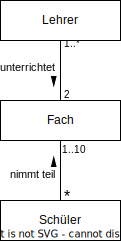
\includegraphics{Bilder/Kapitel-4/klassendiagramm_lehrer_fach_schueler.pdf}
	\caption[Ein zum Objektdiagramm aus Abb.~\ref{fig:objektdiagramm} gehöriges Klassen\-diagramm]{Ein zum Objektdiagramm aus Abbildung~\ref{fig:objektdiagramm} gehöriges Klassen\-diagramm}
	\label{fig:klassendiagramm_zu_objektdiagramm}
\end{figure}

\vspace{\baselineskip} %%% für Druck

Das Klassendiagramm spezifiziert, welche Objekte mit welchen anderen Objekten in welchen Arten von Beziehungen stehen dürfen. Es gibt somit die Regeln vor, anhand derer bestimmt werden kann, ob \marginline{Objekt\-konstellationen}
\textit{Objektkonstellationen} (Menge von Objekten mit oder ohne Verbindungen untereinander) gültig oder ungültig sind. Eine Objektkonstellation ist dann gültig, wenn sie alle durch das Klassendiagramm festgelegten Bedingungen erfüllt, andernfalls ist sie ungültig. Wenn mit einer Objekt\-konstel\-la\-tion wie in Abbildung~\ref{fig:objektdiagramm} begonnen wird, von der die Domänenexperten gesagt haben, dass diese eine adäquate Modellierung der Realweltzusammenhänge darstellt, und sie damit gültig sein soll, muss man das Klassendiagramm und seine Regeln ent\-sprechend so konstruieren, dass alle gültigen Objektkonstellationen der Spezi\-fi\-kation entsprechen. In der Praxis findet häufig aber auch der umgekehrte Weg statt: Man beginnt mit einem Klassendiagramm und erstellt auf dieser Grundlage – im Prinzip nur zu Diskussions- oder Prüfzwecken mit den Domänenexperten – gültige und ungültige Objektkonstellationen.

\vspace{1.4mm} %%% für Druck

Das Klassendiagramm in Abbildung~\ref{fig:klassendiagramm_zu_objektdiagramm} beinhaltet die drei Klassen \sttpUMLText{Lehrer}, \sttpUMLText{Fach} und \sttpUMLText{Schüler}, da für das Objektdiagramm aus Abbildung~\ref{fig:objektdiagramm} Lehrer-Objekte, Fach-Objekte und Schüler-Objekte benötigt werden. Wie zwischen Objekten werden Beziehungen zwischen Klassen in UML durch eine durchgezogene Linie zwischen den Klassen dargestellt. Eine solche Beziehung zwischen Klassen nennt man eine \textit{\mbox{Assoziation}}
\marginline{Assoziationen}
(engl. association). 

\vspace{1.4mm} %%% für Druck

Die Angaben mit Zahlen und Sternchen (*) an den Assoziationsenden in Abbildung~\ref{fig:klassendiagramm_zu_objektdiagramm} heißen \textit{Multiplizitäten}.
\marginline{Multiplizitäten}
Die Multiplizitäten geben an, mit wie vielen anderen Objekten (in Bezug auf die betrachtete Assoziation) die Objekte einer Klasse in Beziehungen stehen können bzw. müssen. Multiplizitäten werden in der Form \sttpUMLText{untereGrenze..obereGrenze} angegeben (\zb \sttpUMLText{1..10}), wobei die untere Grenze die minimale Anzahl und die obere Grenze die maximale Anzahl angibt. Sind untere und obere Grenze identisch, genügt die Angabe eines Werts (\zb \sttpUMLText{2} als Abkürzung für \sttpUMLText{2..2}). Neben der Angabe natürlicher Zahlen kennt die UML in Multiplizitäten noch die Angaben \sttpUMLText{0} und \sttpUMLText{*}. Die \sttpUMLText{0} kann nur als untere Grenze verwendet werden (\zb \sttpUMLText{0..6}) und bedeutet, dass kein verbundenes Objekt gefordert wird. Das Sternchen-Symbol (\sttpUMLText{*}) kann als obere Grenze verwendet werden (wie bei \sttpUMLText{1..*} an der Assoziation \sttpUMLText{unterrichtet}) oder alleine stehen (wie auf der Seite von Schüler an der Assoziation \sttpUMLText{nimmt teil}). Letztere Form ist eine Abkürzung für \sttpUMLText{0..*}, insofern bildet das \sttpUMLText{*} auch hier die obere Grenze. Es bedeutet unbegrenzt viele, wobei unbegrenzt nur nach oben gilt, die angegebene untere Grenze wird durch das Sternchen nicht beeinflusst. Zum Beispiel wären vier Objekte durch die Angabe \sttpUMLText{5..*} nicht abgedeckt, 37~allerdings schon und genauso auch zwei Millionen. 

\vspace{1.4mm} %%% für Druck

Das Lesen
\marginline{Bedeutung von Multiplizitäten}
und das sprachlich adäquate Erläutern der Bedeutung von Multiplizitäten in Klassendiagrammen ist nicht ganz einfach. Ein entscheidender Aspekt, mit dem UML-Anfänger oft Schwierigkeiten haben: Das Klassendiagramm zeigt Klassen und ihre mit Multiplizitäten versehenen Beziehungen zueinander. Die durch die Multiplizitäten modellierten Bedingungen beziehen sich aber nicht auf die Klassen, sondern auf die Objekte dieser Klassen. Man modelliert also Klassen-Beziehungen obwohl man Objekt-Beziehungen spezifizieren möchte.

\vspace{1.4mm} %%% für Druck

Die zweite Schwierigkeit ist, welche Multiplizität die relevante für eine Aussage ist, denn jede Assoziation zwischen zwei Klassen besitzt zwei Multiplizitäten. Wir verlassen kurz Abbildung~\ref{fig:klassendiagramm_zu_objektdiagramm} und wechseln auf ein kleineres Beispiel. Abbildung~\ref{fig:klassendiagramm_und_objektkonstellationen} zeigt oben wieder eine \sttpUMLText{unterrichtet}-Assoziation zwischen einer \sttpUMLText{Lehrer}-Klasse und einer \sttpUMLText{Fach}-Klasse. Die Assoziation weist eine Multiplizität \sttpUMLText{2} auf der Seite der \sttpUMLText{Lehrer}-Klasse und eine Multiplizität \sttpUMLText{3} auf der Seite der \sttpUMLText{Fach}-Klasse auf. 

\pagebreak %%% für Druck

\begin{figure}[h!]
	\vspace{8mm} %%% für Druck
	\centering
	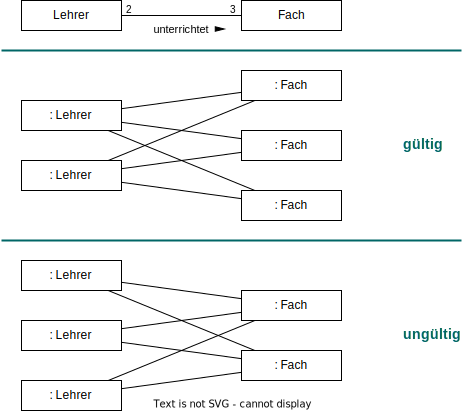
\includegraphics{Bilder/Kapitel-4/objektkonstellation_gueltig_ungueltig.pdf}
	\caption[Klassendiagramm, gültige und ungültige Objektkonstellation]{Ein Klassendiagramm (oben), eine gültige Objektkonstellation (Mitte) und eine ungültige Objektkonstellation (unten)}
	\label{fig:klassendiagramm_und_objektkonstellationen}
\end{figure}

Für Aussagen über die gültigen Verbindungen von Lehrer-Objekten muss (für manchen wenig intuitiv) die Multiplizität auf Seite der \sttpUMLText{Fach}-Klasse betrachtet werden und umgekehrt. Jedes Lehrer-Objekt ist also mit drei Fach-Objekten verbunden und nicht mit zwei und jedes Fach-Objekt mit zwei Lehrer-Objekten und nicht mit drei. Abbildung~\ref{fig:klassendiagramm_und_objektkonstellationen} zeigt in der Mitte eine gültige Objektkonstellation bezüglich des Klassendiagramms und unten eine ungültige Objektkonstellation. Bei Letzterer wurden die Multiplizitäten verkehrt herum gelesen.

Im Prinzip müssten die Assoziationsnamen aus dem Klassendiagramm (in unserem Beispiel \sttpUMLText{unterrichtet}) als Verbindungsnamen in die Objektdiagramme übernommen werden. Aus Übersichtlichkeitsgründen werden in Objektdiagrammen Verbindungsnamen aber häufig nicht angegeben, zumal in der Praxis Objektdiagramme selten ohne Vorliegen bzw. Kenntnis des zugehörigen Klassendiagramms eingesetzt werden, in dem die Assoziationsnamen Auskunft über die Art der Beziehungen zwischen den Objekten geben.

Die dritte Schwierigkeit bei der Interpretation von Multiplizitäten ist zu erkennen, dass mit einer mit Multiplizitäten versehenen Assoziation nicht eine, sondern \textbf{zwei} Aussagen verbunden sind. Die eine Aussage benennt, welche Bedingungen für die Objekte der einen an der Assoziation beteiligten Klasse gelten, die andere gibt an, welche Bedingungen für die Objekte der anderen Klasse gelten. 

\pagebreak %%% für Druck

Wir betrachten weiterhin Abbildung~\ref{fig:klassendiagramm_und_objektkonstellationen}. Es ist nicht möglich, die Bedeutung der beiden Multiplizitäten der Assoziation \sttpUMLText{unterrichtet} in nur einer Formulierung unter\-zubringen. Sätze wie „zwei Lehrer-Objekte stehen in Beziehung mit drei Fach-Objekten“ sind schlichtweg nicht eindeutig. Zwar würden sie durchaus die gültige Objektkonstellation in Abbildung~\ref{fig:klassendiagramm_und_objektkonstellationen} Mitte beschreiben, jedoch auch eine ungültige Objektkonstellation wie in Abbildung~\ref{fig:ungueltige_objektkonstellation} und alle weiteren Beziehungen, in denen zwei Lehrer-Objekte und drei Fach-Objekte vorkommen.

\begin{figure}[h!]
	\centering
	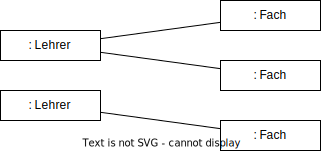
\includegraphics{Bilder/Kapitel-4/ungueltige_objektkonstellation.pdf}
	\caption[Eine ungültige Objektkonstellation zu Abb.~\ref{fig:klassendiagramm_und_objektkonstellationen}]{Eine bezüglich des Klassendiagramms in Abbildung~\ref{fig:klassendiagramm_und_objektkonstellationen} ungültige Objektkonstellation}
	\label{fig:ungueltige_objektkonstellation}
\end{figure}

Es  müssen daher 
\marginline{Multiplizitäten sprachlich ausdrücken}
zwei Aussagen zur Beschreibung der Assoziation verwendet werden: 1. Jedes Lehrer-Objekt ist mit genau drei Fach-Objekten verbunden, 2. Jedes Fach-Objekt (wiederum) ist mit genau zwei Lehrer-Objekten verbunden. Wichtig ist hierbei auch die Formulierung \textbf{jedes} Objekt: Die Vorgaben des Klassendiagramms bezüglich der Verbindungen der Objekte einer Klasse zu anderen Objekten gelten für \textbf{jedes} Objekt dieser Klasse, nicht nur für ein Objekt oder eine bestimmte Teilmenge der Objekte! Wichtig ist auch, dass Multiplizitäten nichts über die \textbf{absolute} Anzahl von Objekten in der Objektkonstellation aussagen.

\sttpHinweiskasten{1.0}{ein vs. jedes}{In der deutschen Sprache verwenden wir in manchen Situationen, in denen wir eigentlich jeder/jede meinen, die Formulierung ein/eine. Zum Beispiel ist mit der Aussage „eine Fichte ist ein Nadelbaum“ vermutlich in den meisten Fällen gemeint, dass es sich bei jeder Fichte um einen Nadelbaum handelt und nicht nur bei einer konkreten Fichte. Eindeutig ist dies aber nicht. Für die sprachliche Erläuterung von Multiplizitäten sollten Sie explizit die Formulierung \textbf{jedes} Objekt verwenden.}

\pagebreak

Kehren wir zum Objektdiagramm aus Abbildung~\ref{fig:objektdiagramm} und zum Klassendiagramm aus Abbildung~\ref{fig:klassendiagramm_zu_objektdiagramm} zurück. 

\begin{center}
	\begin{minipage}[c]{.6\linewidth} 
		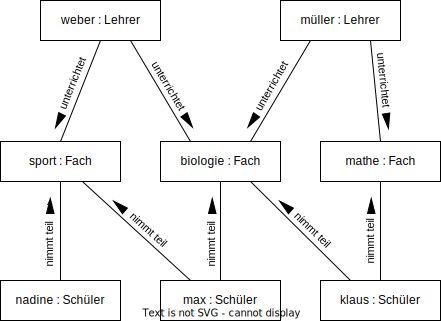
\includegraphics[scale=0.7]{Bilder/Kapitel-4/objektdiagramm_lehrer_fach_schueler.pdf}
	\end{minipage}
	\hspace{.1\linewidth}% Abstand zwischen den beiden Bildern
	\begin{minipage}[c]{.2\linewidth}
		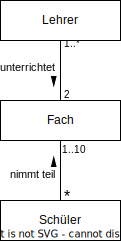
\includegraphics[scale=0.7]{Bilder/Kapitel-4/klassendiagramm_lehrer_fach_schueler.pdf}
	\end{minipage}
\end{center}

Folgende Bedingungen stellt das Klassendiagramm an gültige Objektkonstellationen:
\begin{itemize}
	\item Jedes Lehrer-Objekt ist bezüglich der Verbindungsart \sttpUMLText{unterrichtet} mit genau zwei Fach-Objekten verbunden (Multiplizität: \sttpUMLText{2}). In Realweltterminologie heißt das: Jeder Lehrer unterrichtet genau zwei Fächer.
	\item Jedes Fach-Objekt ist bezüglich der Verbindungsart \sttpUMLText{unterrichtet} mit mindestens einem Lehrer-Objekt verbunden (Multiplizität: \sttpUMLText{1..*}). Realwelt\-termi\-no\-logie: Jedes Fach wird von mindestens einem Lehrer unterrichtet. Auf Grundlage des Objektdiagramms in Abbildung~\ref{fig:objektdiagramm} hätten wir diese Multiplizität durchaus auch weiter einschränken können, denn in Abb.~\ref{fig:objektdiagramm} ist ein konkretes Fach-Objekt entweder mit genau einem Lehrer-Objekt (\sttpUMLText{sport}, \sttpUMLText{mathe}) oder mit genau zwei Lehrer-Objekten (\sttpUMLText{biologie}) verbunden. Die Multiplizität im Klassendiagramm in Abb.~\ref{fig:klassendiagramm_zu_objektdiagramm} hätte also auch \sttpUMLText{1..2} lauten können. Üblicherweise versucht man Multiplizitäten – insbesondere die obere Grenze einer Multiplizität – nicht von Beginn an aufgrund weniger beispielhafter Objekt\-konstellationen zu sehr einzuschränken, da häufig in der weiteren Diskussion mit Domänenexperten doch noch abweichende Fälle auftauchen. Insofern finden sich in den frühen Versionen eines Domänenmodells sehr häufig die Angaben \sttpUMLText{*} oder \sttpUMLText{1..*}. 
	\item Jedes Fach-Objekt ist bezüglich der Verbindungsart \sttpUMLText{nimmt teil} mit beliebig vielen Schüler-Objekten verbunden (Multiplizität \sttpUMLText{*}). Realweltterminologie: An einem (Unterrichts)Fach können beliebig viele (auch keiner!) Schüler teilnehmen. 
	\item Jedes Schüler-Objekt ist bezüglich der Verbindungsart \sttpUMLText{nimmt teil} mit ein bis zehn Fach-Objekten verbunden (Multiplizität: \sttpUMLText{1..10}). Realweltterminologie: Jeder Schüler nimmt mindestens an einem, aber maximal an zehn Fächern teil. 
\end{itemize}

Da wir das Klassendiagramm auf Grundlage der als gültig definierten Objektkonstellation aus Abb.~\ref{fig:objektdiagramm} entsprechend konstruiert haben, erfüllt das Objektdiagramm in Abb.~\ref{fig:objektdiagramm} alle Regeln des Klassendiagramms aus Abb.~\ref{fig:klassendiagramm_zu_objektdiagramm}. Sofern im weiteren Verlauf des Softwareentwicklungsprojekts weitere Objektkonstellationen der Realwelt auftauchen, die ebenfalls gültig sein sollen, muss die aktuelle Version des Klassendiagramms geprüft und unter Umständen angepasst werden.

\minisec{Mehrere Assoziationen zwischen Klassen}

In unserem bisherigen Beispiel waren zwei Objekte immer nur über genau eine Verbindung miteinander verbunden. In der Realwelt existieren aber auch Konstellationen, bei denen zwei Objekte über unterschiedliche Beziehungsarten miteinander verbunden sind. Dies lässt sich auch in der UML modellieren. Abbildung~\ref{fig:assoziationen_zwischen_klassen} zeigt eine Klasse \sttpUMLText{Person} und eine Klasse \sttpUMLText{Glücksspielautomat}. Beide sind durch zwei verschiedene Assoziationen verbunden. Die obere Assoziation bildet ab, dass Personen (in der Realwelt) an Spielautomaten spielen. Die untere Assoziation bildet ab, dass es Personen gibt, die für die Wartung von Spielautomaten zuständig sind. Je nach Art der Beziehung übernehmen Spielautomat-Objekte und Person-Objekte unterschiedliche \marginline{Rollen}
\textit{Rollen}. Achtung: Das ist hier ein anderer Rollenbegriff als der aus Lektion 1.

\vspace{-\baselineskip} %%% für Druck

\begin{figure}[h!]
	\centering
	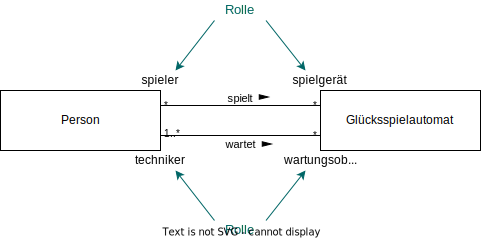
\includegraphics{Bilder/Kapitel-4/assoziationen_zwischen_klassen.pdf}
	\caption{Mehrere Assoziationen zwischen zwei Klassen}
	\label{fig:assoziationen_zwischen_klassen}
\end{figure}

Die  Rollenbezeichnungen können zusätzlich zum Assoziationsnamen an der Assoziation notiert werden, sind aber optional. Rollenbezeichnungen sind im Übrigen nicht auf Situationen beschränkt, in denen mehrere Assoziationen zwischen Klassen modelliert werden sollen. Jede Assoziation kann durch Rollenangaben ergänzt werden. Häufig lassen sich aber schon aus dem Assoziationsnamen die Rollen erschließen, sodass bei nur einer Assoziation zwischen zwei Klassen auf die Angabe von Rollen oft verzichtet wird. Existieren mehrere Assoziationen zwischen Klassen, wie in unserem Spielautomaten-Beispiel, muss aber mindestens eine der beiden Angaben (Assoziationsname oder Rollenbezeichnungen) vorhanden sein, um die Assoziationen unterscheidbar zu halten. 

% Die Grafik ist breiter als die Textbreite.
\begin{figure}[h!]
	\centering
	\includegraphics{Bilder/Kapitel-4/assoziationen_zwischen_klassen_objektdiagramm.pdf}
	\caption[Ein gültiges Objektdiagramm zu Abb.~\ref{fig:assoziationen_zwischen_klassen}]{Ein gültiges Objektdiagramm zu Abbildung~\ref{fig:assoziationen_zwischen_klassen}}
	\label{fig:objektdiagramm_zu_assoziationen_zwischen_klassen}
\end{figure}

Abbildung~\ref{fig:objektdiagramm_zu_assoziationen_zwischen_klassen} zeigt ein Objektdiagramm mit einer gültigen Objektkonstellation bezüglich des Klassendiagramms in Abbildung~\ref{fig:assoziationen_zwischen_klassen}: Sie sehen, dass es Personen geben kann, die an Spielautomaten spielen (Peter), andere die einen Spielautomaten warten (Tom und Mareike), wieder andere, die beides tun (Manfred) und solche, die weder Spieler noch Techniker sind (Hans). All dies lässt das Klassendiagramm aus Abb.~\ref{fig:assoziationen_zwischen_klassen} zu.

\pagebreak %%% für Druck

Abbildung~\ref{fig:tierarzt_tier} zeigt ein weiteres Beispiel für mehrere Assoziationen zwischen Klassen. Zwischen den Klassen \sttpUMLText{Tierarzt} und \sttpUMLText{Tier} gibt es zwei unterschiedliche Beziehungen. Mit der Assoziation \sttpUMLText{impft} soll modelliert werden, dass Tierärzte Tiere impfen. Die Assoziation \sttpUMLText{Jahresuntersuchung} modelliert, dass Tierärzte bei Tieren regelmäßige Vorsorgeuntersuchungen vornehmen. In diesem Beispiel würden sich Rollenbezeichnungen an den beiden Assoziationen nicht sehr voneinander unterscheiden, da das Tier in beiden Fällen eine Art Patient und der Tierarzt eben der Arzt wäre. Man könnte natürlich Rollenbezeichnungen wie \sttpUMLText{impfkandidat}, \sttpUMLText{impfarzt} für die eine Assoziation und \sttpUMLText{patient}, \sttpUMLText{untersuchender} für die andere Assoziation kreieren oder ähnliche voneinander abweichende Formulierungen. Für das Verständnis hilfreicher ist in diesem Beispiel aber der Verzicht auf die Rollenangaben und stattdessen die Verwendung aussagekräftiger Assoziationsnamen. Im Übrigen verwendet man für Assoziationsnamen üblicherweise Verben. Der Assoziationsname \sttpUMLText{Jahresuntersuchung} der unteren Assoziation ist hier aber mal ein Beispiel für einen Fall, in dem ein Nomen als Assoziationsname geeigneter ist als ein Verb.

\begin{figure}[h!]
	\centering
	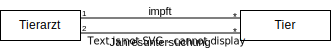
\includegraphics{Bilder/Kapitel-4/tierarzt_tier.pdf}
	\caption[Beispiel für mehrere Assoziationen zwischen Klassen]{Weiteres Beispiel für mehrere Assoziationen zwischen Klassen}
	\label{fig:tierarzt_tier}
\end{figure}

\minisec{Reflexive Assoziationen}

Eine besondere Art von Assoziationen sind sogenannte \textit{reflexive Assoziationen}, die Beziehungen zwischen \textbf{verschiedenen} Objekten \textbf{derselben} Klasse beschreiben. Die Assoziation \sttpUMLText{vertritt} in Abbildung~\ref{fig:assoziation_und_objektkonstellation} oben ist ein Beispiel für eine reflexive Assoziation. Sie beschreibt eine Beziehung zwischen einem Sachbearbeiter-Objekt und anderen Sachbearbeiter-Objekten. Im Beispiel wird modelliert, dass ein Realwelt-Sachbearbeiter durch zwei andere Sachbearbeiter vertreten werden kann (\zb im Urlaubsfall). Abbildung~\ref{fig:assoziation_und_objektkonstellation} unten zeigt eine gültige Objektkonstellation: Der Sachbearbeiter Max steht in seiner Rolle als Verantwortlicher in Verbindungen mit seinen Vertretern den Sachbearbeitern Paul und Hugo. In seiner Rolle als Vertreter steht Max gleichzeitig in Verbindung zur Sachbearbeiterin Sabine, deren Vertretung er übernimmt. In diesem Beispiel ist die Angabe der Rollen für das Verständnis der Beziehungen notwendig. 

\begin{figure}[h!]
	\centering
	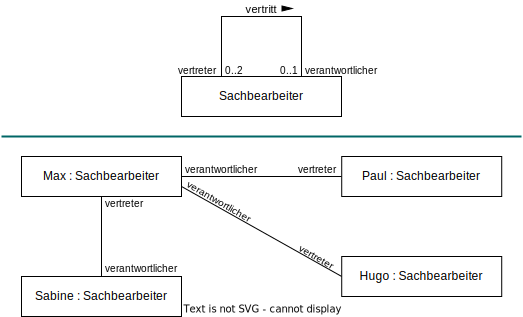
\includegraphics{Bilder/Kapitel-4/sachbearbeiter.pdf}
	\caption[Eine reflexive Assoziation]{Eine reflexive Assoziation (oben) und eine dazu gültige Objekt\-konstellation (unten)}
	\label{fig:assoziation_und_objektkonstellation}
\end{figure}

\minisec{n-äre Beziehungen}
In der Realwelt gibt es Situationen, in denen Objekte von mehr als zwei Klassen miteinander in Beziehung stehen. In der UML drückt man eine solche sogenannte \textit{\mbox{n-äre} Beziehung} zwischen Klassen (\zb drei Klassen: ternär, vier Klassen: quaternär) mit Assoziationen aus, die durch eine Raute verknüpft sind. Abbildung~\ref{fig:tierarzt_tier_krankheit} zeigt ein Beispiel. Zwischen den Klassen \sttpUMLText{Tierarzt}, \sttpUMLText{Tier} und \sttpUMLText{Krankheit} besteht eine Assoziation mit Namen \sttpUMLText{heilt}. Damit soll modelliert werden, dass Tierärzte Tiere von Krankheiten heilen.

\begin{figure}[h!]
	\centering
	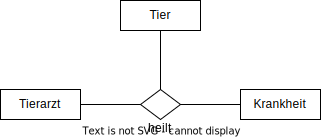
\includegraphics{Bilder/Kapitel-4/tierarzt_tier_krankheit.pdf}
	\caption{Eine Beziehung zwischen drei Klassen}
	\label{fig:tierarzt_tier_krankheit}
\end{figure}

\pagebreak %%% für Druck

Java und viele andere objektorientierte Programmiersprachen unterstützen das Konzept der n-ären Beziehungen nicht, sodass bei der Implementierung solche Assoziationen in mehrere binäre Assoziationen umgewandelt werden müssen. In Domänenmodellen können n-äre Beziehungen aber vorkommen, wenn sie in der Realwelt existieren (und dementsprechend den Domänenexperten geläufig sind), denn Domänenmodelle sollen noch unabhängig sein von jeglichen späteren Implementierungsbedürfnissen.

\minisec{Aggregation und Komposition}
\phantomsection
\label{sec:Kap-3.2.5.3:besondere_assoziationen}

Um weitere besondere Formen von Beziehungen auszudrücken, kennt die UML außer den einfachen Assoziationen, die man mit Assoziationsnamen, Multiplizitäten und Rollen versehen kann, mit der \textit{Aggregation} und der \textit{Komposition} noch zwei spezielle Assoziationen. Mit Aggregation und Komposition lassen sich Teil-Ganzes-Beziehungen modellieren, zum Beispiel ein Einkauf, dessen Teile die einzelnen eingekauften Produkte sind oder ein Haus, das aus mehreren Zimmern besteht. Abbildung~\ref{fig:aggregation_und_komposition} zeigt diese beiden Beispiele. 

\begin{figure}[h!]
	\centering
	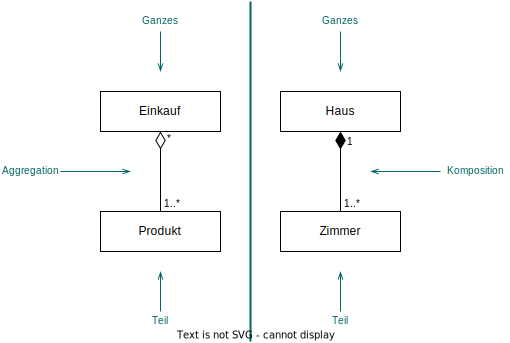
\includegraphics{Bilder/Kapitel-4/aggregation_vs_komposition.pdf}
	\caption[Aggregation und Komposition]{Aggregation (links) und Komposition (rechts)}
	\label{fig:aggregation_und_komposition}
\end{figure}

Aggregationsbeziehungen, wie hier zwischen \sttpUMLText{Einkauf} und \sttpUMLText{Produkt}, und Komposi\-tions\-beziehungen, wie zwischen \sttpUMLText{Haus} und \sttpUMLText{Zimmer}, werden durch eine Raute am Assoziationsende des Ganzes-Elements dargestellt. Die unausgefüllte Raute (Abbildung links) kennzeichnet die Aggregation, die ausgefüllte Raute (Abbildung rechts) die Komposition. Assoziationsnamen werden üblicherweise nicht angegeben, da die Art der Beziehung (\sttpUMLText{„besteht aus“}, \sttpUMLText{„hat“}, \sttpUMLText{„setzt sich zusammen aus“},
\sttpUMLText{„ist} \sttpUMLText{Teil} \sttpUMLText{von“} etc.) schon aus der gewählten Verbindungsform hervorgeht.

Aggregation und Komposition drücken im Vergleich zu einfachen Assoziationen eine stärkere Beziehung zwischen den verbundenen Objekten aus, wobei über die Komposition eine noch engere Beziehung modelliert wird als über die Aggrega\-tion. Die Darstellung als Komposition wird verwendet, wenn die Teile (im Beispiel die Zimmer-Objekte) nicht unabhängig vom Ganzen (Haus-Objekt) existieren können, die Verbindung zwischen dem Ganzen und seinen Teilen also untrennbar ist bzw. sein soll. Dementsprechend darf ein konkretes Teil-Objekt auch nur mit einem einzigen Ganzes-Objekt verbunden sein (Multiplizität \sttpUMLText{1} auf der Seite der Klasse \sttpUMLText{Haus}). In Aggregationsbeziehungen ist dagegen die Existenz der Teile (Produkt-Objekte) auch ohne das Ganze (Einkauf-Objekt) vorgesehen.

\minisec{Assoziationsklassen}
Abbildung~\ref{fig:kind_patenschaft_tier} zeigt ein Beispiel für eine sogenannte \textit{Assoziationsklasse}. Mit einer Assoziationsklasse können die Eigenschaften einer Assoziation und die Eigenschaften einer Klasse kombiniert werden. Das macht es möglich, eine Assoziation -- der man nur Namen, Rollen, Multiplizitäten anfügen kann -- zusätzlich mit Merkmalen einer Klasse, wie zum Beispiel Attributen, auszustatten. Man verwendet Assoziations\-klassen, um Charakteristika abzubilden, die Teil der Beziehung zwischen den beteiligten Objekten sind und sich nicht einer der an der Beziehung beteiligten Klassen zuordnen lassen. In unserem Beispiel spielt für eine Patenschaft, die ein Kind für ein Tier übernimmt, der Zeitraum dieser Patenschaft eine Rolle. Diese Information wird als Attribut modelliert.

\begin{figure}[h!]
	\centering
	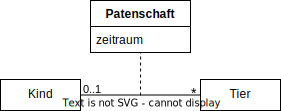
\includegraphics{Bilder/Kapitel-4/kind_patenschaft_tier.pdf}
	\caption{Eine Assoziationsklasse}
	\label{fig:kind_patenschaft_tier}
\end{figure}

In der UML-Darstellung wird die Assoziationsklasse mit einer gestrichelten Linie an die Assoziationslinie angebunden. Der Name der Assoziationsklasse und der Name der Assoziation müssen identisch sein, wobei letzterer optional ist. Ähnlich wie bei den n-ären Beziehungen müssen Assoziationsklassen-Beziehungen für die Implementierung in andere Beziehungsformen umgewandelt werden, da die objektorientierten Programmiersprachen das Konzept der Assoziationsklasse nicht unterstützen. In \mbox{Domänenmodellen} sind sie aber häufig zu finden.

\minisec{Generalisierung}

Lassen Sie uns zum Schluss des Kapitels noch eine weitere besondere Beziehungsform ansehen, die eine wichtige Rolle in der Objektorientierung spielt. Um (hierarchische) Realweltklassifikationen, sogenannte Taxonomien, abbilden zu können, gibt es das Konzept der \textit{Generalisierung}. Abbildung~\ref{fig:generalisierungsbeziehungen} zeigt die UML-Syntax für die Modellierung von Generalisierungsbeziehungen.

\begin{figure}[h!]
	\centering
	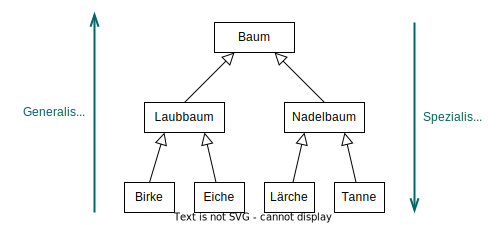
\includegraphics{Bilder/Kapitel-4/generalisierungsbeziehungen.pdf}
	\caption{Generalisierungsbeziehungen}
	\label{fig:generalisierungsbeziehungen}
\end{figure}

Laubbäume und Nadelbäume sind spezielle Formen von Bäumen. In der Terminologie der Objektorientierung sagt man, sie sind \textit{Spezialisierungen} von Bäumen. Die Begriffe Generalisierung und Spezialisierung meinen dasselbe Konzept, sie beschreiben es nur aus zwei unterschiedlichen Richtungen. Ausgehend von der Klasse \sttpUMLText{Baum} sind die Klassen \sttpUMLText{Laubbaum} und \sttpUMLText{Nadelbaum} Spezialisierungen. Aus Richtung der Klasse \sttpUMLText{Laubbaum} bzw. \sttpUMLText{Nadelbaum} betrachtet, ist die Klasse \sttpUMLText{Baum} eine Generalisierung. Die Generalisierungsklasse nennt man auch \textit{Oberklasse},
\marginline{Ober- und Unterklasse}
die Spezialisierungsklasse heißt \textit{Unterklasse}. Generalisierungsbeziehungen sind also Beziehungen zwischen Ober\-klassen und Unterklassen. In der UML wird Generalisierung/Spezialisierung durch einen Pfeil mit einer unausgefüllten Dreiecksspitze auf der Seite der Oberklasse modelliert.

In der Klasse \sttpUMLText{Baum} aus Abb.~\ref{fig:generalisierungsbeziehungen} könnte definiert sein, dass jedes Baum-Objekt eine Wurzel, einen Stamm und Zweige besitzt. Diese Charakteristika der Ober\-klasse gelten in Generalisierungsbeziehungen auch für die Objekte der Unterklassen. In der Terminologie der objektorientierten Programmierung sagt man, die Ober\-klasse \textit{vererbt} Eigenschaften an ihre Unterklasse(n). Die Unterklasse wiederum kann Eigenschaften zu dem Ererbten hinzufügen oder auch Ererbtes verändern, um die Spezialisierung zu charakterisieren. Zum Beispiel charakterisiert einen Laubbaum, dass er Blätter hat, während ein Nadelbaum keine Blätter, sondern Nadeln besitzt. Charakteristisch für eine Birke als Spezialisierung eines Laubbaums ist zum Beispiel die besondere Färbung des Stamms, während eine Eiche, die ebenfalls eine Spezialisierung eines Laubbaums ist, sich durch die Form ihrer Blätter auszeichnet. Auf einer konzeptuellen Ebene ist ein Laubbaum-Objekt aus unserem Beispiel nicht nur ein Laubbaum (hat Blätter) sondern gleichzeitig auch ein Baum (hat Wurzel, Stamm und Zweige). Ein Birke-Objekt ist gleichzeitig eine Birke (Stamm ist weiß), ein Laubbaum (hat Blätter) und ein Baum (hat Wurzel, Stamm und Zweige). 

%--- Kapitel 4.4 KommLit
\clearpage
\section{Kommentierte Literatur}
\label{sec:Kap-4.4}


\sttpKommLitItem{Lahres/Raýman/Strich}{2018}{Objektorientierte Programmierung}{lah18}{Bilder/Buchcover/Buchcover_Lahres_Rayman_Strich.png}{}
{Häufig sind Bücher zu objektorientierter Programmierung eigentlich nur Einführungen in konkrete objektorientierte Programmiersprachen. Das ist hier nicht so. Das Buch beschäftigt sich sehr systematisch und konzeptionell und dabei gut verständlich mit den Prinzipien, der Methodik, den Elementen und dem Einsatz objektorientierter Softwareentwicklung, unabhängig von konkreten Programmiersprachen. Den Schwerpunkt bilden Implementierungsaspekte, dennoch findet man auch viele Informationen zur Objektorientierung im Allgemeinen und Aspekten der objektorientierten Realweltmodellierung. Neben Kapitel~2, das die Objektorientierung im Vergleich zu anderen Programmiermethodiken vorstellt, ist für die Inhalte dieser Lektion vor allem Kapitel~4 relevant. Dieses stellt die Konzepte Objekt und Klasse, ihre Charakteristika und ihre Einsatzmöglichkeiten umfassend vor.}

\sttpKommLitItem{Kecher/Salvanos/Hoffmann-Elbern}{2018}{UML~2.5}{kec18}{Bilder/Buchcover/Buchcover_Kecher_Salvanos.jpg}{}
{Das Kapitel zum UML-Klassendiagramm (S.~37~ff.) ist fast hundert Seiten lang. Sämtliche Elemente, die in einem Klassendiagramm vorkommen können, werden hier gut verständlich mit Realweltbeispielen beschrieben. Bei vielen Elementen wird sogar zusätzlich eine mögliche Umsetzung in Programmcode mit angegeben. Für Anfänger besonders hilfreich sind die Hinweise, für welche Modellierungszwecke sich welche Elemente besonders anbieten.}

\sttpKommLitItem{Sommerville}{2018}{Software Engineering}{som18}{Bilder/Buchcover/Buchcover_Sommerville.jpg}{}
{Kapitel~5 des Lehrbuchs stellt verschiedene Modellarten der UML und ihre Einsatzzwecke im Softwareengineering vor, das UML-Klassendiagramm wird in Kapitel~5.3 behandelt. Im Unterschied zu anderen Lehrbüchern beziehen sich die UML-Beispiele in diesem Buch immer auf eines der vier durchgehenden Fallbeispiele, die in Kapitel~1 vorgestellt werden und sich durch alle Themen des Buchs ziehen. Das hat den Vorteil, dass man sich nicht ständig in neue Kontexte einarbeiten muss, wenn man auch andere Softwareengineering-Themen mit diesem Buch lernen möchte; aber auch den Nachteil, dass es nicht immer die am intuitivsten passenden Beispiele für ein konkretes UML-Konzept sind. Insgesamt ist es gerade für Objektorientierung- und UML-Anfänger sehr zu empfehlen, mit mehreren Büchern zu arbeiten, da jede Autorin/ jeder Autor einen etwas (oder auch sehr) anderen Zugang zum Thema hat.}

\sttpKommLitItem{Brügge/Dutoit}{2006}{Objektorientierte Softwaretechnik}{bru06}{Bilder/Buchcover/Buchcover_Bruegge_Dutoit.jpg}{}
{Kapitel~2.3 des Lehrbuchs stellt unter anderem die Begriffe Modellierung, Objekt, Klasse, Datentyp und Domäne vor. Kapitel~2.4 beschäftigt sich mit unterschiedlichen Diagrammarten der UML, unter anderem mit dem Klassendiagramm. Hier wird auf knapp zehn Seiten ein guter erster Einblick in die wichtigsten Aspekte des UML-Klassendiagramms anhand verschiedener Beispiele gegeben. Für eine intensivere Beschäftigung mit Klassendiagrammen – und anderen UML-Diagrammen – sollte man aber immer auch die speziellen UML-Bücher wie \cite{kec18} zu Rate ziehen.}

\sttpKommLitItem{Oestereich/Scheithauer}{2013}{Analyse und Design mit der UML~2.5}{oes13}{Bilder/Buchcover/Buchcover_Oesterreich_Scheithauer.jpg}{}
{Abschnitt~7 (S.~17~ff) enthält eine Einführung in die Objektorientierung mit den wichtigsten Aspekten in Bezug auf Klassen und Objekte.}

